\documentclass[11pt,a4paper,russian,intlimits]{ncc}
\usepackage[utf8]{inputenc}
\usepackage[T2A]{fontenc}
\DeclareUnicodeCharacter{2009}{\,}
\usepackage[margin=2cm]{geometry}

\usepackage{color}

\usepackage{hyperref}
\hypersetup{
    colorlinks=true,
    linkcolor=black,
    filecolor=magenta,
    urlcolor=cyan,
    linktoc=all,
}

\usepackage{graphicx}

% Needed for Asciidoc

\newcommand{\admonition}[2]{\textbf{#1}: {#2}}
\newcommand{\rolered}[1]{ \textcolor{red}{#1} }
\newcommand{\roleblue}[1]{ \textcolor{blue}{#1} }


\renewenvironment{quotation}
{   \leftskip 4em \begin{em} }
{\end{em}\par }

\def\signed#1{{\leavevmode\unskip\nobreak\hfil\penalty50\hskip2em
  \hbox{}\nobreak\hfil\raise-3pt\hbox{(#1)}%
  \parfillskip=0pt \finalhyphendemerits=0 \endgraf}}


\newsavebox\mybox

\newenvironment{aquote}[1]
  {\savebox\mybox{#1}\begin{quotation}}
  {\signed{\usebox\mybox}\end{quotation}}

\newenvironment{tquote}[1]
  {  {\bf #1} \begin{quotation} \\ }
  { \end{quotation} }

%% BOXES: http://tex.stackexchange.com/questions/83930/what-are-the-different-kinds-of-boxes-in-latex
%% ENVIRONMENTS: https://www.sharelatex.com/learn/Environments

\newenvironment{asciidocbox}
  {\leftskip6em\rightskip6em\par}
  {\par}

\newenvironment{titledasciidocbox}[1]
  {\leftskip6em\rightskip6em\par{\bf #1}\vskip-0.6em\par}
  {\par}



%%%%%%%%%%%%%%%%%%%%%%%%%%%%%%%%%%%%%%%%%%%%%%%%%%%%%%%%

%% http://texblog.org/tag/rightskip/


\newenvironment{preamble}
  {}
  {}

%% http://tex.stackexchange.com/questions/99809/box-or-sidebar-for-additional-text
%%
\newenvironment{sidebar}[1][r]
  {\wrapfigure{#1}{0.5\textwidth}\tcolorbox}
  {\endtcolorbox\endwrapfigure}


%%%%%%%%%%

\newenvironment{comment*}
  {\leftskip6em\rightskip6em\par}
  {\par}

  % \newenvironment{remark*}
  % {\leftskip6em\rightskip6em\par}
  % {\par}


%% Dummy environment for testing:

\newenvironment{foo}
  {\bf Foo.\ }
  {}


\newenvironment{foo*}
  {\bf Foo.\ }
  {}


\newenvironment{click}
  {\bf Click.\ }
  {}

\newenvironment{click*}
  {\bf Click.\ }
  {}


% \newenvironment{remark}
%   {\bf Remark.\ }
%   {}

\newenvironment{capsule}
  {\leftskip10em\par}
  {\par}

%%%%%%%%%%%%%%%%%%%%%%%%%%%%%%%%%%%%%%%%%%%%%%%%%%%%%



\title{Ковёр Серпинского, или как я познакомился с шейдерами}

\begin{document}
\maketitle
\tableofcontents
Одним жарким летним днём мне пришла в голову идея научиться рисовать фракталы на OpenGL с шейдерами. В качестве примера я решил взять ковёр Серпинского, как относительно простой в определении и построении фрактал.

\section{Ковер Серпинского}

Ковер Серпинского можно просто получить из обычного квадрата: разделим квадрат на 9 частей и вырежем серединку. Теперь для каждого из восьми оставшихся квадратов сделаем то же самое. Повторив процедуру бесконечное число раз мы получим всюду дырявый квадрат, который и называется ковром Серпинского.


\section{Построение фракталов}

Понятно, что построить всюду дырявый ковер не получится: для определения всех точек, в него не попадающих потребуется сделать бесконечное число итераций. Поэтому мы сделаем просто достаточно много итераций и для каждого пиксела изображения определим, на какой итерации мы его вырезали. По номеру итерации мы определим цвет, в который покрасим этот пиксель.

\section{Шейдеры}

Особенностью построения фракталов заключается в независимости цвета пиксела от цвета других пикселов. Поэтому считать итерации можно параллельно на видеокарте используя шейдер.

Перейдём к написанию кода для шейдера:

\begin{lstlisting}
// shader.glsl

#version 120       // версия glsl

void main() {
    // получаем координату точки на текстуре
    vec2 p = gl_TexCoord[0].xy;

    // число итераций
    int iterations = 5;
    int i;
    for(i=0; i<iterations; ++i) {
        // увеличим наш квадрат 1х1 в 3 раза
        p = 3.0 * p;

        // если попали в середину, то прекращаем итерации
        if (p.x > 1.0 && p.x < 2.0 &&
            p.y > 1.0 && p.y < 2.0)
             break;

        // снова возвращаемся к квадрату 1x1
        p -= vec2(ivec2(p));
    }

    // определяем оттенок серого по числу итераций
    vec3 color = vec3(float(i) / float(iterations));
    gl_FragColor = vec4(color, 1.0);
}
\end{lstlisting}

А теперь напишем на C простенькую программу, чтобы используя этот шейдер нарисовать ковёр Серпинского:

\begin{lstlisting}
// main.c

#include <GL/glew.h>
#include <GL/glut.h>
#include <stdio.h>

GLuint program;
void render();
char* readFile();

int main(int argc, char** argv) {
    glutInit(&argc, argv);
    glutInitDisplayMode(GLUT_RGBA | GLUT_DOUBLE | GLUT_MULTISAMPLE);
    glutInitWindowSize(500, 500);
    glutInitWindowPosition(50, 50);
    glutCreateWindow("Sierpinski carpet");
    glutDisplayFunc(render);
    glewInit();

    // компиляция и линковка шейдера
    program = glCreateProgram();
    GLuint shader = glCreateShader(GL_FRAGMENT_SHADER);
    const char* buffer = readFile("shader.glsl");
    glShaderSource(shader, 1, &buffer, 0);
    glCompileShader(shader);
    glAttachShader(program, shader);
    glLinkProgram(program);

    glutMainLoop();
}

void render() {
    glUseProgram(program);

    // рисуем квадрат на всё окно
    // именно его текстуру будет рисовать шейдер
    glBegin(GL_POLYGON);
    glTexCoord2f(1, 0);
    glVertex2f(1, -1);
    glTexCoord2f(1, 1);
    glVertex2f(1, 1);
    glTexCoord2f(0, 1);
    glVertex2f(-1, 1);
    glTexCoord2f(0, 0);
    glVertex2f(-1, -1);
    glEnd();

    glUseProgram(0);

    glutSwapBuffers();
}


char * readFile(const char* fname) {
    FILE* fp;
    long lSize;
    char* buffer;
    
    fp = fopen (fname, "r");
    if(!fp) {
        perror(fname);
        exit(1);
    }

    fseek(fp, 0L, SEEK_END);
    lSize = ftell(fp);
    rewind(fp);

    /* выделяем память для текста + 1 для нулевого байта */
    buffer = calloc(sizeof(char), lSize+1);
    if(!buffer) {
        fclose(fp);
        fputs("memory alloc fails", stderr);
        exit(1);
    }

    /* копируем содержимое файла в буфер */
    if(1!=fread(buffer, lSize, 1, fp)) {
      fclose(fp);
      free(buffer);
      fputs("entire read fails", stderr);
      exit(1);
    }

    fclose(fp);
    return buffer;
}
\end{lstlisting}

В результате получаем вот такую красоту:

\begin{figure}[h]
    \center
    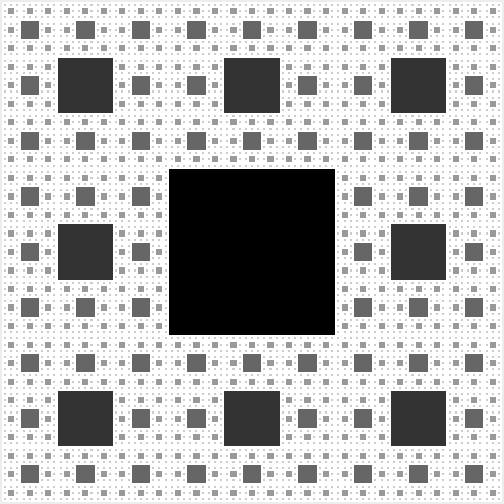
\includegraphics[width=.5\textwidth]{2015-09-06-sierpinski-carpet-and-shader-sierpinski.png}
    \caption{Ковёр Серпинского}
\end{figure}

Код можно взять \href{https://github.com/citrux/sierpinski-carpet}{здесь}.

\end{document}